\documentclass{article}

\usepackage{tikz} 
\usetikzlibrary{automata, positioning, arrows} 

\usepackage{amsthm}
\usepackage{amsfonts}
\usepackage{amsmath}
\usepackage{amssymb}
\usepackage{fullpage}
\usepackage{color}
\usepackage{parskip}
\usepackage{hyperref}
\usepackage{graphicx}

  \hypersetup{
    colorlinks = true,
    urlcolor = blue,
    linkcolor= blue,
    citecolor= blue,
    filecolor= blue,
    }
    
\usepackage{listings}
\usepackage[utf8]{inputenc}                                                    
\usepackage[T1]{fontenc}      
\usepackage{enumitem}                                                 

\definecolor{dkgreen}{rgb}{0,0.6,0}
\definecolor{gray}{rgb}{0.5,0.5,0.5}
\definecolor{mauve}{rgb}{0.58,0,0.82}

\lstset{frame=tb,
  language=haskell,
  aboveskip=3mm,
  belowskip=3mm,
  showstringspaces=false,
  columns=flexible,
  basicstyle={\small\ttfamily},
  numbers=none,
  numberstyle=\tiny\color{gray},
  keywordstyle=\color{blue},
  commentstyle=\color{dkgreen},
  stringstyle=\color{mauve},
  breaklines=true,
  breakatwhitespace=true,
  tabsize=3
}

\newtheoremstyle{theorem}
  {\topsep} {\topsep} {\itshape\/} {0pt} {\bfseries} {.} {5pt plus 1pt minus 1pt} {}
\theoremstyle{theorem} 
   \newtheorem{theorem}{Theorem}[section]
   \newtheorem{corollary}[theorem]{Corollary}
   \newtheorem{lemma}[theorem]{Lemma}
   \newtheorem{proposition}[theorem]{Proposition}
\theoremstyle{definition}
   \newtheorem{definition}[theorem]{Definition}
   \newtheorem{example}[theorem]{Example}
\theoremstyle{remark}    
  \newtheorem{remark}[theorem]{Remark}

\lstdefinelanguage{PythonDFARun}{
    keywords={def, for, in, if, return},
    keywordstyle=\color{blue}\bfseries,
    morekeywords={self},
    keywordstyle=[2]\color{purple},
    morekeywords=[2]{self},
    stringstyle=\color{red},
    commentstyle=\color{gray},
    identifierstyle=\color{black},
    sensitive=true
}

\lstset{
    language=PythonDFARun,
    basicstyle=\ttfamily\footnotesize,
    frame=single,
    showstringspaces=false,
    tabsize=4
}

\title{CPSC-354 Report}
\author{Jeffrey Bok  \\ Chapman University}
\date{\today} 

\begin{document}

\maketitle

\begin{abstract}

\end{abstract}

\setcounter{tocdepth}{3}
\tableofcontents

\section{Introduction}\label{intro}

\section{Week by Week}\label{homework}

\subsection{Week 1}
\subsubsection{Homework}

What is the MU Puzzle and how do you "solve" it?:

The MU puzzle is a logic puzzle created by Douglas Hofstadter in his 1979 book "Gödel, Escher, Bach: An Eternal Golden Braid." It's designed to illustrate concepts about formal systems, computability, and the limits of rule-based reasoning. The rules are below:

Rule I: If a string ends in I, you can add U to the end (xI → xIU)\newline
Rule II: If you have Mx, you can make Mxx (double everything after M)\newline
Rule III: If you find III anywhere in your string, you can replace it with U (xIIIy → xUy)\newline
Rule IV: If you find UU anywhere in your string, you can remove it (xUUy → xy)

To "solve" the puzzle, you try to apply a combination of rules step by step, creating new strings. 
Eventually, you'll find that MU can never be reached because the rules never allow you to remove the odd number of \texttt{I}'s needed to get zero. 

\subsubsection{Exploration}
Hofstadter used this puzzle to demonstrate how formal systems can have inherent limitations - some statements that seem like they should be provable within a system are actually unprovable. This connects to Gödel's incompleteness theorems and fundamental questions about the nature of mathematical truth and computation.

Programming languages are formal systems, just like the MU puzzle. They have:

\begin{itemize}
\item Syntax rules (what constitutes valid code)
\item Transformation rules (how expressions evaluate)  
\item Semantic constraints (what programs can actually compute)
\end{itemize}

The MU puzzle demonstrates that even simple rule sets can have hidden limitations - similarly, programming languages have inherent computational boundaries.

\subsubsection{Questions}
1. The impossibility of reaching "MU" from "MI" is provable, yet someone working within the system might not realize this. How does this relate to the halting problem and undecidable questions in programming?

\subsection{Week 2}
\subsubsection{Homework}
    Consider the following list of ARSs:\newline
    \begin{enumerate}
    \item $A = \{\}$.
    \item $A = \{a\}$ and $R = \{\}$.
    \item $A = \{a\}$ and $R = \{(a,a)\}$.
    \item $A = \{a,b,c\}$ and $R = \{(a,b),(a,c)\}$.
    \item $A = \{a,b\}$ and $R = \{(a,a),(a,b)\}$.
    \item $A = \{a,b,c\}$ and $R = \{(a,b),(b,b),(a,c)\}$.
    \item $A = \{a,b,c\}$ and $R = \{(a,b),(b,b),(a,c),(c,c)\}$.
    \end{enumerate}
    
    Draw a picture for each of the ARSs above. Are the ARSs terminating? Are they confluent? Do they have unique normal forms?

    Try to find an example of an ARS for each of the possible 8 combinations. Draw pictures of these examples.

        
    \paragraph{ARS 1: $A = \{\}$}
    \begin{center}
    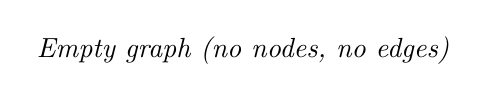
\begin{tikzpicture}
        \node at (0,0) {\textit{Empty graph (no nodes, no edges)}};
    \end{tikzpicture}
    \end{center}
    \textbf{Terminating:} YES \quad \textbf{Confluent:} YES \quad \textbf{Unique Normal Forms:} YES
    
    \paragraph{ARS 2: $A = \{a\}$, $R = \{\}$}
    \begin{center}
    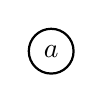
\begin{tikzpicture}[node distance=2cm, auto, thick]
        \node[circle, draw] (a) {$a$};
    \end{tikzpicture}
    \end{center}
    \textbf{Terminating:} YES \quad \textbf{Confluent:} YES \quad \textbf{Unique Normal Forms:} YES
    
    \paragraph{ARS 3: $A = \{a\}$, $R = \{(a,a)\}$}
    \begin{center}
    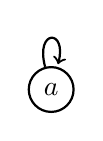
\begin{tikzpicture}[node distance=2cm, auto, thick, -latex]
        \node[circle, draw] (a) {$a$};
        \path (a) edge[loop above] (a);
    \end{tikzpicture}
    \end{center}
    \textbf{Terminating:} NO \quad \textbf{Confluent:} YES \quad \textbf{Unique Normal Forms:} NO
    
    \paragraph{ARS 4: $A = \{a,b,c\}$, $R = \{(a,b),(a,c)\}$}
    \begin{center}
    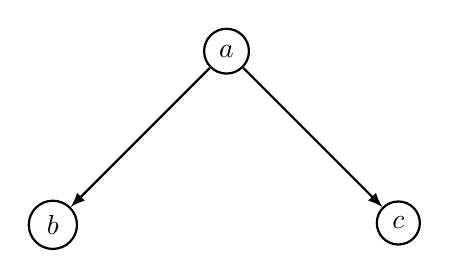
\begin{tikzpicture}[node distance=2.5cm, auto, thick, -latex]
        \node[circle, draw] (a) {$a$};
        \node[circle, draw] (b) [below left=of a] {$b$};
        \node[circle, draw] (c) [below right=of a] {$c$};
        
        \path (a) edge (b);
        \path (a) edge (c);
    \end{tikzpicture}
    \end{center}
    \textbf{Terminating:} YES \quad \textbf{Confluent:} NO \quad \textbf{Unique Normal Forms:} NO
    
    \paragraph{ARS 5: $A = \{a,b\}$, $R = \{(a,a),(a,b)\}$}
    \begin{center}
    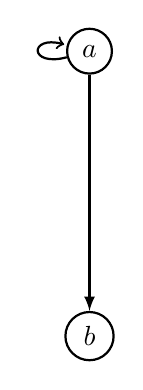
\begin{tikzpicture}[node distance=3cm, auto, thick, -latex]
        \node[circle, draw] (a) {$a$};
        \node[circle, draw] (b) [below=of a] {$b$};
        
        \path (a) edge[loop left] (a);
        \path (a) edge (b);
    \end{tikzpicture}
    \end{center}
    \textbf{Terminating:} NO \quad \textbf{Confluent:} NO \quad \textbf{Unique Normal Forms:} NO
    
    \paragraph{ARS 6: $A = \{a,b,c\}$, $R = \{(a,b),(b,b),(a,c)\}$}
    \begin{center}
    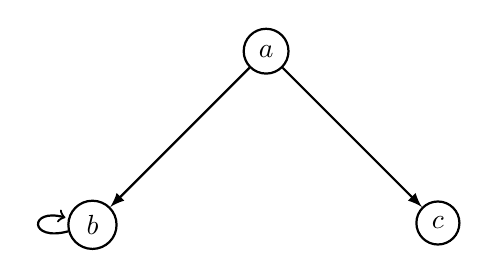
\begin{tikzpicture}[node distance=2.5cm, auto, thick, -latex]
        \node[circle, draw] (a) {$a$};
        \node[circle, draw] (b) [below left=of a] {$b$};
        \node[circle, draw] (c) [below right=of a] {$c$};
        
        \path (a) edge (b);
        \path (a) edge (c);
        \path (b) edge[loop left] (b);
    \end{tikzpicture}
    \end{center}
    \textbf{Terminating:} NO \quad \textbf{Confluent:} NO \quad \textbf{Unique Normal Forms:} NO
    
    \paragraph{ARS 7: $A = \{a,b,c\}$, $R = \{(a,b),(b,b),(a,c),(c,c)\}$}
    \begin{center}
    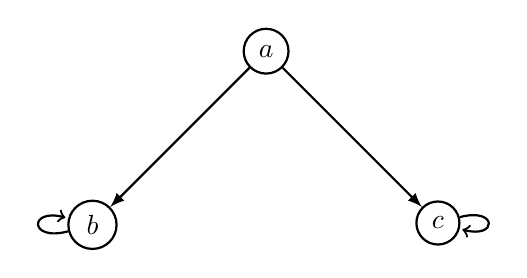
\begin{tikzpicture}[node distance=2.5cm, auto, thick, -latex]
        \node[circle, draw] (a) {$a$};
        \node[circle, draw] (b) [below left=of a] {$b$};
        \node[circle, draw] (c) [below right=of a] {$c$};
        
        \path (a) edge (b);
        \path (a) edge (c);
        \path (b) edge[loop left] (b);
        \path (c) edge[loop right] (c);
    \end{tikzpicture}
    \end{center}
    \textbf{Terminating:} NO \quad \textbf{Confluent:} NO \quad \textbf{Unique Normal Forms:} NO

    \paragraph{8 Combinations Table}
    \begin{center}
        \begin{tabular}{|c|c|c|l|}
        \hline
        \textbf{Confluent} & \textbf{Terminating} & \textbf{Unique NF} & \textbf{Example} \\
        \hline
        True & True & True & $A = \{a\}$, $R = \{\}$ \\
        True & True & False & $A = \{\}$, $R = \{\}$ \\
        True & False & True & $A = \{a,b\}$, $R = \{(a,b),(b,b)\}$ \\
        True & False & False & $A = \{a\}$, $R = \{(a,a)\}$ \\
        False & True & True & $A = \{a,b,c,d\}$, $R = \{(a,b),(a,c),(c,d)\}$ \\
        False & True & False & $A = \{a,b,c\}$, $R = \{(a,b),(a,c)\}$ \\
        False & False & True & $A = \{a,b,c\}$, $R = \{(a,b),(b,a),(a,c),(c,a)\}$ \\
        False & False & False & $A = \{a,b,c\}$, $R = \{(a,b),(b,b),(a,c)\}$ \\
        \hline
        \end{tabular}
    \end{center}

    \paragraph{Examples for 8 Combinations}

    \subparagraph{Example 1: Confluent=T, Terminating=T, Unique Normal Forms=T}
    $A = \{a\}$, $R = \{\}$
    \begin{center}
    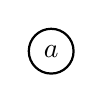
\begin{tikzpicture}[node distance=2cm, auto, thick]
        \node[circle, draw] (a) {$a$};
    \end{tikzpicture}
    \end{center}

    \subparagraph{Example 2: Confluent=T, Terminating=T, Unique Normal Forms=F}
    $A = \{\}$, $R = \{\}$
    \begin{center}
    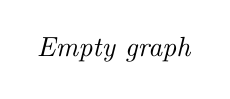
\begin{tikzpicture}
        \node at (0,0) {\textit{Empty graph}};
    \end{tikzpicture}
    \end{center}

    \subparagraph{Example 3: Confluent=T, Terminating=F, Unique Normal Forms=T}
    $A = \{a,b\}$, $R = \{(a,b),(b,b)\}$
    \begin{center}
    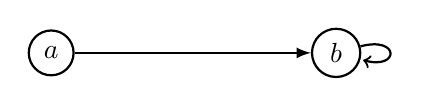
\begin{tikzpicture}[node distance=3cm, auto, thick, -latex]
        \node[circle, draw] (a) {$a$};
        \node[circle, draw] (b) [right=of a] {$b$};
        
        \path (a) edge (b);
        \path (b) edge[loop right] (b);
    \end{tikzpicture}
    \end{center}

    \subparagraph{Example 4: Confluent=T, Terminating=F, Unique Normal Forms=F}
    $A = \{a\}$, $R = \{(a,a)\}$
    \begin{center}
    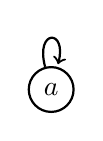
\begin{tikzpicture}[node distance=2cm, auto, thick, -latex]
        \node[circle, draw] (a) {$a$};
        \path (a) edge[loop above] (a);
    \end{tikzpicture}
    \end{center}

    \subparagraph{Example 5: Confluent=F, Terminating=T, Unique Normal Forms=T}
    $A = \{a,b,c,d\}$, $R = \{(a,b),(a,c),(c,d)\}$
    \begin{center}
        \begin{tikzpicture}[node distance=2.5cm, auto, thick, -latex]
            \node[circle, draw] (a) {$a$};
            \node[circle, draw] (b) [below left=of a] {$b$};
            \node[circle, draw] (c) [below right=of a] {$c$};
            \node[circle, draw] (d) [below=of c] {$d$};
            
            \path (a) edge (b);
            \path (a) edge (c);
            \path (c) edge (d);
        \end{tikzpicture}
    \end{center}

    \subparagraph{Example 6: Confluent=F, Terminating=T, Unique Normal Forms=F}
    $A = \{a,b,c\}$, $R = \{(a,b),(a,c)\}$
    \begin{center}
        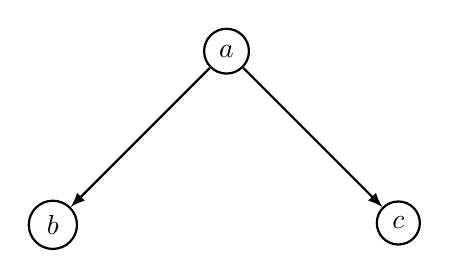
\begin{tikzpicture}[node distance=2.5cm, auto, thick, -latex]
            \node[circle, draw] (a) {$a$};
            \node[circle, draw] (b) [below left=of a] {$b$};
            \node[circle, draw] (c) [below right=of a] {$c$};
            
            \path (a) edge (b);
            \path (a) edge (c);
        \end{tikzpicture}
    \end{center}

    \subparagraph{Example 7: Confluent=F, Terminating=F, Unique Normal Forms=T}
    $A = \{a,b,c\}$, $R = \{(a,b),(b,a),(a,c),(c,a)\}$
    \begin{center}
    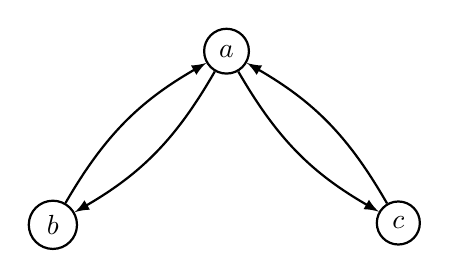
\begin{tikzpicture}[node distance=2.5cm, auto, thick, -latex]
        \node[circle, draw] (a) {$a$};
        \node[circle, draw] (b) [below left=of a] {$b$};
        \node[circle, draw] (c) [below right=of a] {$c$};
        
        \path (a) edge[bend left=15] (b);
        \path (b) edge[bend left=15] (a);
        \path (a) edge[bend right=15] (c);
        \path (c) edge[bend right=15] (a);
    \end{tikzpicture}
    \end{center}

    \subparagraph{Example 8: Confluent=F, Terminating=F, Unique Normal Forms=F}
    $A = \{a,b,c\}$, $R = \{(a,b),(b,b),(a,c)\}$
    \begin{center}
    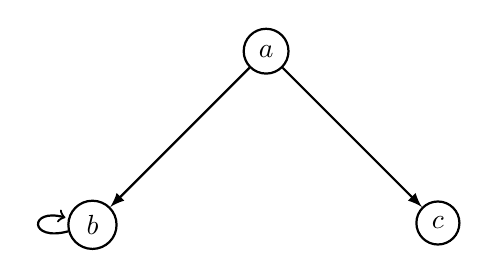
\begin{tikzpicture}[node distance=2.5cm, auto, thick, -latex]
        \node[circle, draw] (a) {$a$};
        \node[circle, draw] (b) [below left=of a] {$b$};
        \node[circle, draw] (c) [below right=of a] {$c$};
        
        \path (a) edge (b);
        \path (a) edge (c);
        \path (b) edge[loop left] (b);
    \end{tikzpicture}
    \end{center}

    \subsubsection{Exploration}
    Abstract Reduction Systems provide a mathematical foundation for understanding computation and rewriting. The properties of termination, confluence, and unique normal forms are fundamental to understanding how programming languages behave:
    
    \begin{itemize}
    \item \textbf{Termination} ensures that computations eventually halt
    \item \textbf{Confluence} guarantees that the order of operations doesn't affect the final result
    \item \textbf{Unique Normal Forms} means every expression has a single, well-defined simplified form
    \end{itemize}
    
    These concepts directly apply to programming language design, where we want predictable evaluation strategies and guaranteed termination for certain classes of programs.
    
    \subsubsection{Questions}
    1. How do the termination properties of ARSs relate to the halting problem in computation?\newline
    2. Why might a programming language designer prefer confluent systems over non-confluent ones?\newline

\subsection{Week 3}
\subsubsection{Homework}
Consider the rewrite rules:
\begin{itemize}
\item ab $\to$ ba
\item ba $\to$ ab  
\item aa $\to$ (empty string)
\item b $\to$ (empty string)
\end{itemize}

\subsubsection{Sample Reductions}
\textbf{Reducing abba:}

abba $\to$ baba (using ab $\to$ ba)

baba $\to$ bbaa (using ab $\to$ ba)

bbaa $\to$ baa (using b $\to$ empty)

baa $\to$ aa (using b $\to$ empty)

aa $\to$ empty (using aa $\to$ empty)

\textbf{Reducing bababa:}

bababa $\to$ bbaaaba (using ab $\to$ ba twice)

bbaaaba $\to$ baaaba (using b $\to$ empty)

baaaba $\to$ aaaba (using b $\to$ empty)

aaaba $\to$ aba (using aa $\to$ empty)

aba $\to$ baa (using ab $\to$ ba)

baa $\to$ aa (using b $\to$ empty)

aa $\to$ empty (using aa $\to$ empty)

\subsubsection{Analysis}
\textbf{Why is the ARS not terminating?}

The first two rules ab $\to$ ba and ba $\to$ ab create cycles. You can apply these rules forever, going back and forth between ab and ba.

\textbf{Find two strings that are not equivalent. How many non-equivalent strings can you find?}

Two strings that are not equivalent: "a" and "empty string". The string "a" cannot be reduced further, while other strings can reduce to empty.

\textbf{Equivalence classes and normal forms:}
There are exactly 2 equivalence classes:
\begin{enumerate}
\item Strings that reduce to empty string
\item Strings that reduce to "a"
\end{enumerate}

The normal forms are: empty string and "a"

\textbf{Modified terminating ARS:}
To make it terminating, always eliminate b's first, then eliminate aa's, then do swapping only if needed.

\textbf{Questions about strings that can be answered using the ARS:}
\begin{enumerate}
\item "Given a string, does it contain an even number of a's?"
\item "Given a string, does it contain an odd number of a's?"
\item "Are two strings equivalent under this rewrite system?"
\end{enumerate}

\subsection{Exercise 5b}
\subsubsection{Modified Rewrite Rules}
Same as Exercise 5, but change aa $\to$ empty to aa $\to$ a:
\begin{itemize}
\item ab $\to$ ba
\item ba $\to$ ab  
\item aa $\to$ a (pairs of a become single a)
\item b $\to$ (empty string)
\end{itemize}

\subsubsection{Sample Reductions}
\textbf{Reducing abba:}

abba $\to$ baba (using ab $\to$ ba)

baba $\to$ bbaa (using ab $\to$ ba)

bbaa $\to$ baa (using b $\to$ empty)

baa $\to$ aa (using b $\to$ empty)

aa $\to$ a (using aa $\to$ a)

\textbf{Reducing bababa:}

bababa $\to$ bbaaaba (using ab $\to$ ba twice)

bbaaaba $\to$ baaaba (using b $\to$ empty)

baaaba $\to$ aaaba (using b $\to$ empty)

aaaba $\to$ aaba (using aa $\to$ a)

aaba $\to$ abaa (using ab $\to$ ba)

abaa $\to$ baaa (using ab $\to$ ba)

baaa $\to$ aaa (using b $\to$ empty)

aaa $\to$ aa (using aa $\to$ a)

aa $\to$ a (using aa $\to$ a)

\subsubsection{Analysis}
\textbf{Why the ARS is not terminating:}
Same as Exercise 5 - the rules ab $\to$ ba and ba $\to$ ab create infinite cycles.

\textbf{Non-equivalent strings:}
Two strings that are not equivalent: "a" and "empty string". We can find exactly 2 non-equivalent strings.

\textbf{Equivalence classes and normal forms:}
There are exactly 2 equivalence classes:
\begin{enumerate}
\item Strings with even number of a's $\to$ reduce to empty
\item Strings with odd number of a's $\to$ reduce to "a"
\end{enumerate}

The normal forms are: empty string and "a"

\textbf{Modified terminating ARS:}
To make it terminating, use the same priority as Exercise 5:
\begin{enumerate}
\item b $\to$ empty (eliminate all b's first)
\item aa $\to$ a (reduce pairs of a's)
\item ab $\to$ ba (only if needed)
\end{enumerate}

\textbf{Questions about strings that can be answered using the ARS:}
\begin{enumerate}
\item "Given a string, does it contain an even number of a's?"
\item "Given a string, does it contain an odd number of a's?"
\item "Are two strings equivalent under this rewrite system?"
\end{enumerate}

\subsubsection{Exploration}
\subsubsection{Questions}
\begin{enumerate}
\item If two completely different sets of rewrite rules (Exercise 5 vs 5b) produce the same equivalence classes, what does this tell us about the relationship between implementation and specification in computer science?

\item If "abab" and "bbaa" are equivalent under this system, but clearly different as strings, what does "equivalence" really mean? Is mathematical equivalence different from everyday sameness?

\end{enumerate}

\subsection{Week 4}
\subsubsection{Homework}
\subsubsection{Exploration}
\subsubsection{Questions}

\subsection{Week 5}
\subsubsection{Homework}
\subsubsection{Exploration}
\subsubsection{Questions}

\subsection{Week 6}
\subsubsection{Homework}
\subsubsection{Exploration}
\subsubsection{Questions}

\subsection{Week 7}
\subsubsection{Homework}
\subsubsection{Exploration}
\subsubsection{Questions}

\subsection{Week 8}
\subsubsection{Homework}

\textbf{Natural Number Game - Tutorial World: Levels 5-8}

\paragraph{Level 5: Simplifying with \texttt{add\_zero}}
Prove that $a + (b + 0) + (c + 0) = a + b + c$.

\begin{lstlisting}[language=haskell]
rw [add_zero]
rw [add_zero]
rfl
\end{lstlisting}

\paragraph{Level 6: Targeted rewriting}
Prove that $a + (b + 0) + (c + 0) = a + b + c$ using explicit arguments.

\begin{lstlisting}[language=haskell]
rw [add_zero c]
rw [add_zero b]
rfl
\end{lstlisting}

\paragraph{Level 7: \texttt{succ\_eq\_add\_one}}
Prove that for all natural numbers $n$, $\text{succ}(n) = n + 1$.

\begin{lstlisting}[language=haskell]
rw [one_eq_succ_zero]
rw [add_succ]
rw [add_zero]
rfl
\end{lstlisting}

\paragraph{Level 8: Proving $2 + 2 = 4$}
Prove that $2 + 2 = 4$.

\begin{lstlisting}[language=haskell]
nth_rewrite 2 [two_eq_succ_one]
rw [add_succ]
rw [one_eq_succ_zero]
rw [add_succ]
rw [add_zero]
rw [<- three_eq_succ_two]
rw [<- four_eq_succ_three]
rfl
\end{lstlisting}

\subsubsection{Natural Language Proof}

\textbf{Level 8: Proving $2 + 2 = 4$}

\begin{proof}
We want to prove that $2 + 2 = 4$ using only the Peano axioms and previously established theorems about natural numbers.

We begin by expanding the second $2$ in the left-hand side using its definition. By the theorem \texttt{two\_eq\_succ\_one}, we know that $2 = \text{succ}(1)$. Rewriting the second occurrence of $2$, we obtain:
$$2 + \text{succ}(1) = 4$$

Next, we apply the fundamental recursion axiom for addition, \texttt{add\_succ}, which states that for any natural numbers $a$ and $b$, we have $a + \text{succ}(b) = \text{succ}(a + b)$. Applying this axiom gives us:
$$\text{succ}(2 + 1) = 4$$

Now we expand $1$ using its definition. By \texttt{one\_eq\_succ\_zero}, we know that $1 = \text{succ}(0)$. Substituting this yields:
$$\text{succ}(2 + \text{succ}(0)) = 4$$

We apply \texttt{add\_succ} again to the inner addition:
$$\text{succ}(\text{succ}(2 + 0)) = 4$$

By the base case axiom for addition, \texttt{add\_zero}, which states that $n + 0 = n$ for any natural number $n$, we can simplify $2 + 0$ to $2$:
$$\text{succ}(\text{succ}(2)) = 4$$

Now we recognize this expression in terms of known number definitions. By the definition \texttt{three\_eq\_succ\_two}, we know that $3 = \text{succ}(2)$. Using this in reverse (indicated by the backwards arrow in the formal proof), we can rewrite $\text{succ}(2)$ as $3$:
$$\text{succ}(3) = 4$$

Finally, by the definition \texttt{four\_eq\_succ\_three}, we know that $4 = \text{succ}(3)$. Using this in reverse, we obtain:
$$4 = 4$$

This is true by the reflexivity of equality: any object is equal to itself.

Therefore, $2 + 2 = 4$.
\end{proof}

\subsubsection{Exploration}

The proof of $2 + 2 = 4$ is a remarkable example of how even the simplest arithmetic facts require rigorous justification when building mathematics from first principles. Several profound insights emerge from this exercise:

\begin{itemize}
\item \textbf{Numbers as constructions}: In the Peano axioms, numbers are not primitive objects but are constructed iteratively from zero using the successor function. The number $2$ is defined as $\text{succ}(\text{succ}(0))$, $3$ as $\text{succ}(2)$, and $4$ as $\text{succ}(3)$. This constructive approach ensures that all natural numbers can be built systematically.

\item \textbf{Addition as recursion}: Addition is not defined by a lookup table but by two recursive rules: the base case $n + 0 = n$ and the recursive case $n + \text{succ}(m) = \text{succ}(n + m)$. The proof of $2 + 2 = 4$ essentially "executes" this recursive definition step by step.

\item \textbf{The role of definitions}: Much of the proof consists of unfolding and refolding definitions. We expand $2$ into $\text{succ}(1)$, then $1$ into $\text{succ}(0)$, perform the addition, and finally recognize the result as $3$ and then $4$. This shows that definitions are not just abbreviations but active components of reasoning.

\item \textbf{Computational content of proofs}: This proof has a computational interpretation. Each rewrite step corresponds to a computation step, and the entire proof traces the execution of the addition algorithm. This connection between proofs and programs is central to the Curry-Howard correspondence.

\item \textbf{Nothing is obvious in formal systems}: What seems trivial in everyday mathematics ($2 + 2 = 4$) requires multiple logical steps when formalized. This explicitness is both a strength (eliminates ambiguity and hidden assumptions) and a weakness (can obscure high-level mathematical intuition).
\end{itemize}

This exercise bridges the gap between our intuitive understanding of arithmetic and the formal foundations required for computer-verified mathematics and programming language semantics.

\subsubsection{Questions}

\begin{enumerate}
\item Why does proving $2 + 2 = 4$ require eight steps when it seems inherently true?

\item When should a programming language prioritize precision over simplicity?
\end{enumerate}

\subsection{Week 9}
\subsubsection{Homework}
\subsubsection{Exploration}
\subsubsection{Questions}

\subsection{Week 10}
\subsubsection{Homework}
\subsubsection{Exploration}
\subsubsection{Questions}

\subsection{Week 11}
\subsubsection{Homework}
\subsubsection{Exploration}
\subsubsection{Questions}

\section{Synthesis}

\section{Evidence of Participation}

\section{Conclusion}\label{conclusion}

\begin{thebibliography}{9}
\end{thebibliography}

\end{document}
